\newchapter{commissioning}{Setup and Commissioning of the PFF System}

This is the introductory text.

\newsection{fontSetup}{Feedforward Controller (FONT5a Board)}

\subsection{Cabling Setup}
\label{ss:fontCables}

\subsection{Implementation of PFF Algorithm in Firmware}
\label{ss:pffFirmware}

Not using arcsin in phase reconstruction - effect

Gain conversion factor

\subsection{DAQ and Setup Parameters}
\label{ss:fontDAQ}

gain
                                                                                                           
filter weights

timing delays

saturate rather than overflow output

Interleaved mode


\subsection{ADC Droop Correction}
\label{ss:droopCorr}

The droop in the response of the FONT5 ADCs, as most clearly seen in the output of the diode channel in Figure \ref{f:diodeDroop} (although it also effects the mixer channel), is not an issue for the work the FONT group does at ATF2 where the signals are well approximated by delta functions separated by \(\sim\)100~ns. Although the droop has been seen previously, its significance for the continuous microsecond length pulse at CTF3 had not been considered because of this.

\begin{figure}
  \centering
  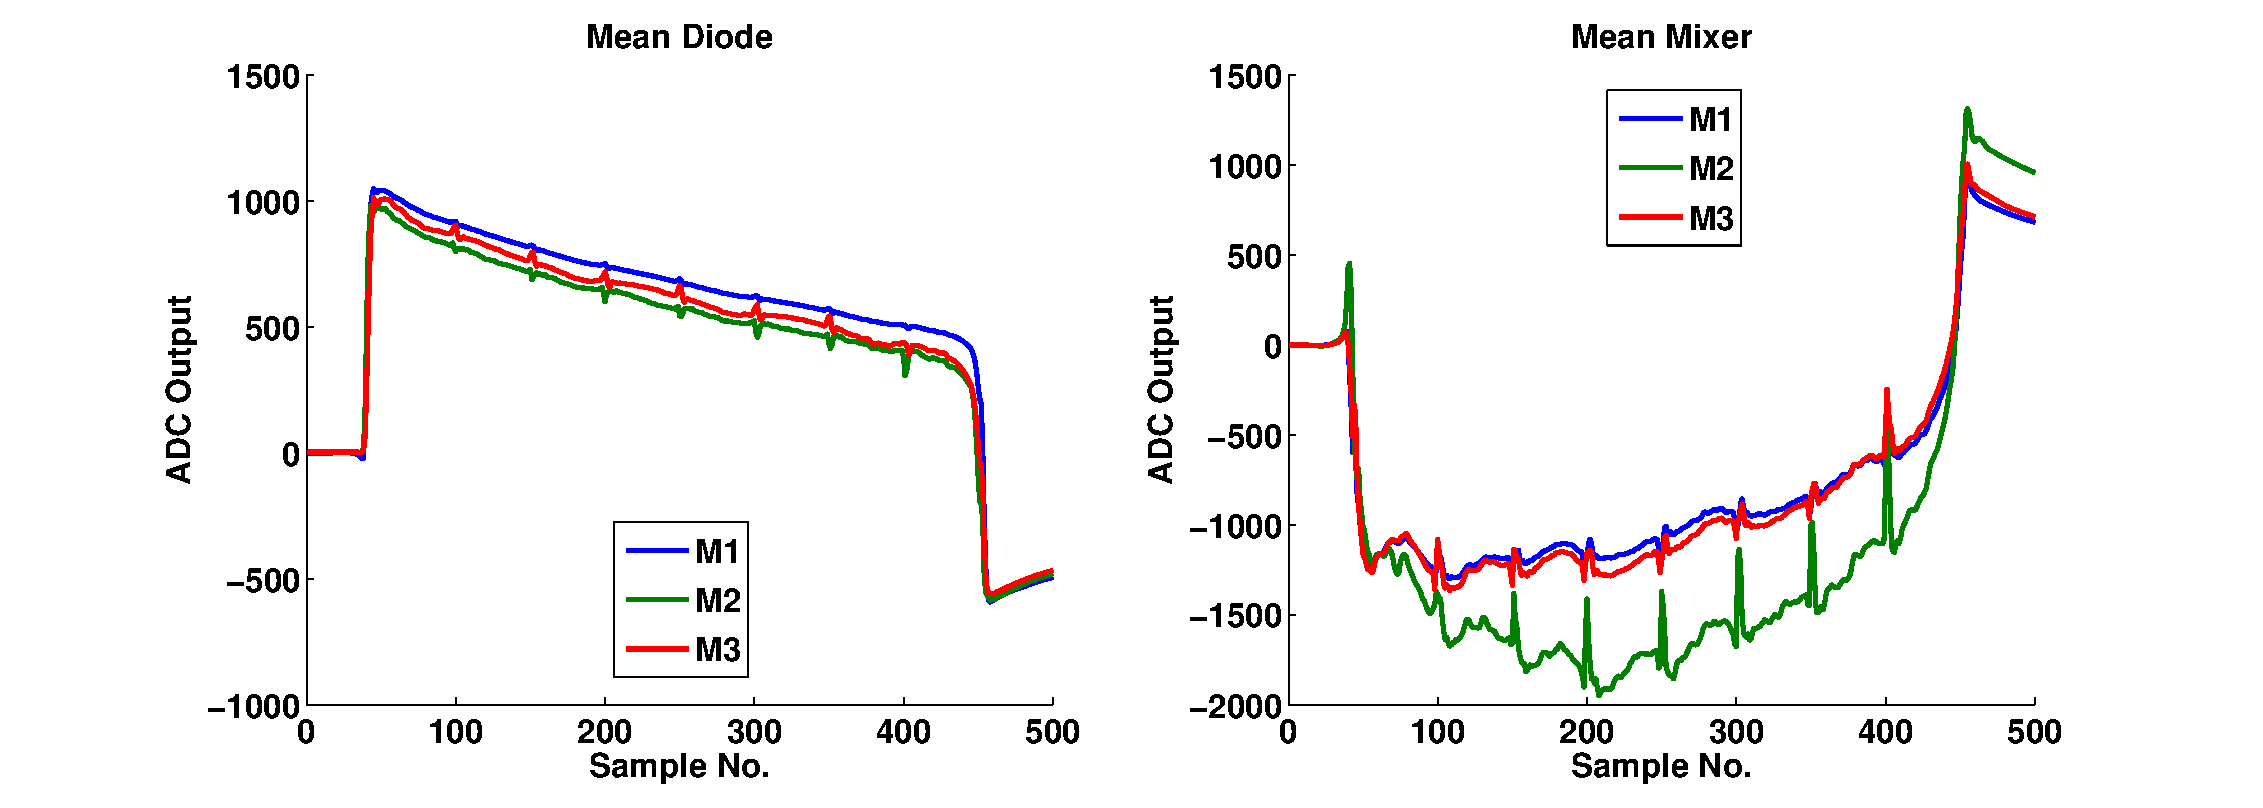
\includegraphics[width=0.9\textwidth]{Figures/commissioning/diodeDroop}
  \caption{Mean diode and mixer output with no filter.}
  \label{f:diodeDroop}
\end{figure}

The droop emerges as a result of the use of AC coupling on the ADC input transformers for electrical isolation. This involves using a capacitor, the current across which is dependent on \({dV}/{dt}\) (\(V\) being voltage and \(t\) time), to remove the DC component from a signal. In particular for the diode channel, which should be a square wave, the output is increasingly well described by a DC signal on the flat top as you move away from the leading edge of the pulse, with the capacitor causing droop in the response as a result.

In the simplest case the droop should be well described by an exponential decay of the form \(A\exp\left(-t/T\right)\). The droop makes it difficult to perform calibrations and measurements on the data and one way in which it could be removed in offline analysis is by determining the decay constants, \(T\), for each of the ADCs on the FONT5 board. To avoid the influence of beam effects tests were done in Oxford using a generated 10~\(\mu\)s DC pulse.

\begin{figure}
  \centering
  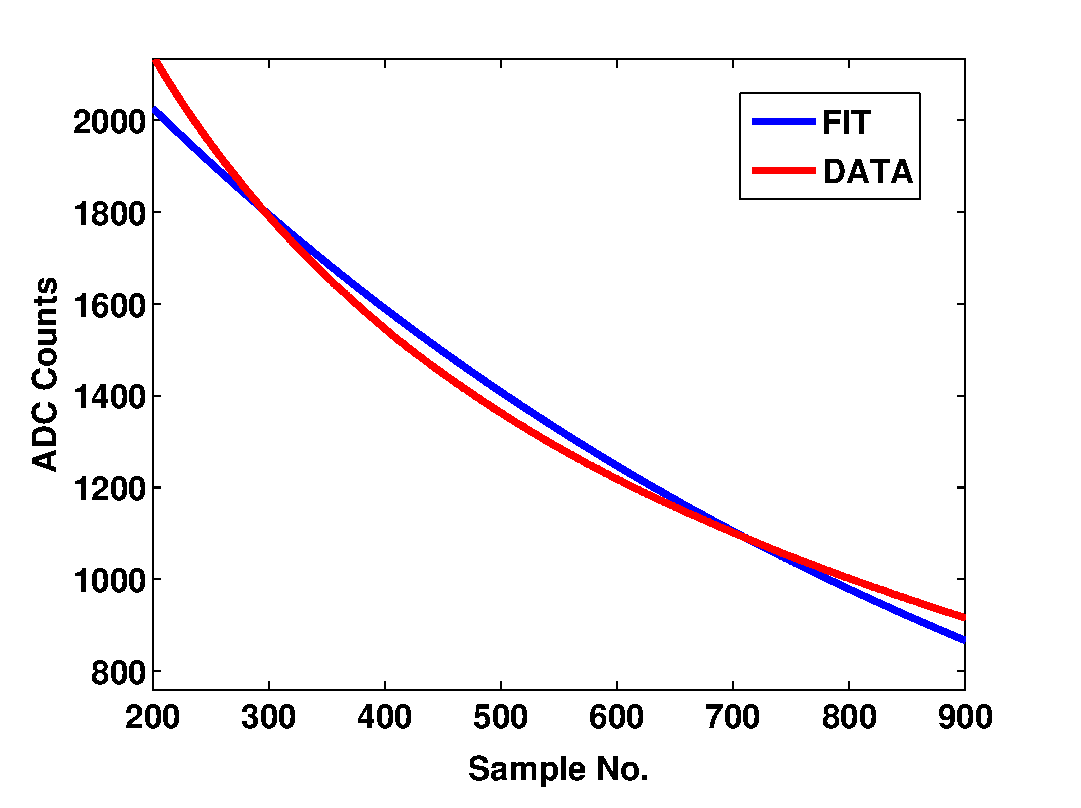
\includegraphics[width=0.45\textwidth]{Figures/commissioning/droopFit}
  \caption{Attempted exponential fit to the ADC droop.}
  \label{f:droopFit}
\end{figure}

Unfortunately, as can be seen in Figure \ref{f:droopFit} which shows an example of an exponential fit for one ADC, although the fits return good \(R^{2}\) values it is clear that the slope of the exponential curve is not a good match for the slope of the data. This is perhaps not unexpected as the ferrite cores used in the transformers have many non-linear properties. In fact, by using a fit with two exponential terms it is possible to obtain a perfect match to the data but at this point the complexity of the fit would make any attempt to remove the droop in real beam data in this way spurious.

Instead, changes will be made to the currently in development FONT5a board hardware and firmware to greatly reduce the scale of the droop. Different transformers will be used to reduce the droop rate by up to a factor of fifty and in addition digital filtering will be implemented in firmware to smooth out and reduce the remaining droop component even further. It is expected that after these changes the droop will be small enough to not have a detrimental effect on the performance of the phase feedforward system. 


\newsection{amplifierSetup}{Amplifier}

Make point that all effects here much smaller than phase monitors/phase propagation and although important to highlight them no attempts yet made to correct them or take them in to account in simulations.

Amplifier versions:

First version (nov 2014) 350 V (check)

2nd version  (jul 2015) 650 V - double FETs

3rd version: 1200 V with combiner module (?) not pursued

\subsection{Installation}
\label{ss:ampInstallation}


Amplifier inputs:

Trigger from FONT5a board

DAC1 and DAC2 from FONT5a board


Amplifier outputs:

4 drive signals - one for each strip. Sent to downstream end of kicker (why?)

4 terminators

Amplifier on time monitoring

Monitoring of each amplifier output

\begin{figure}
  \centering
  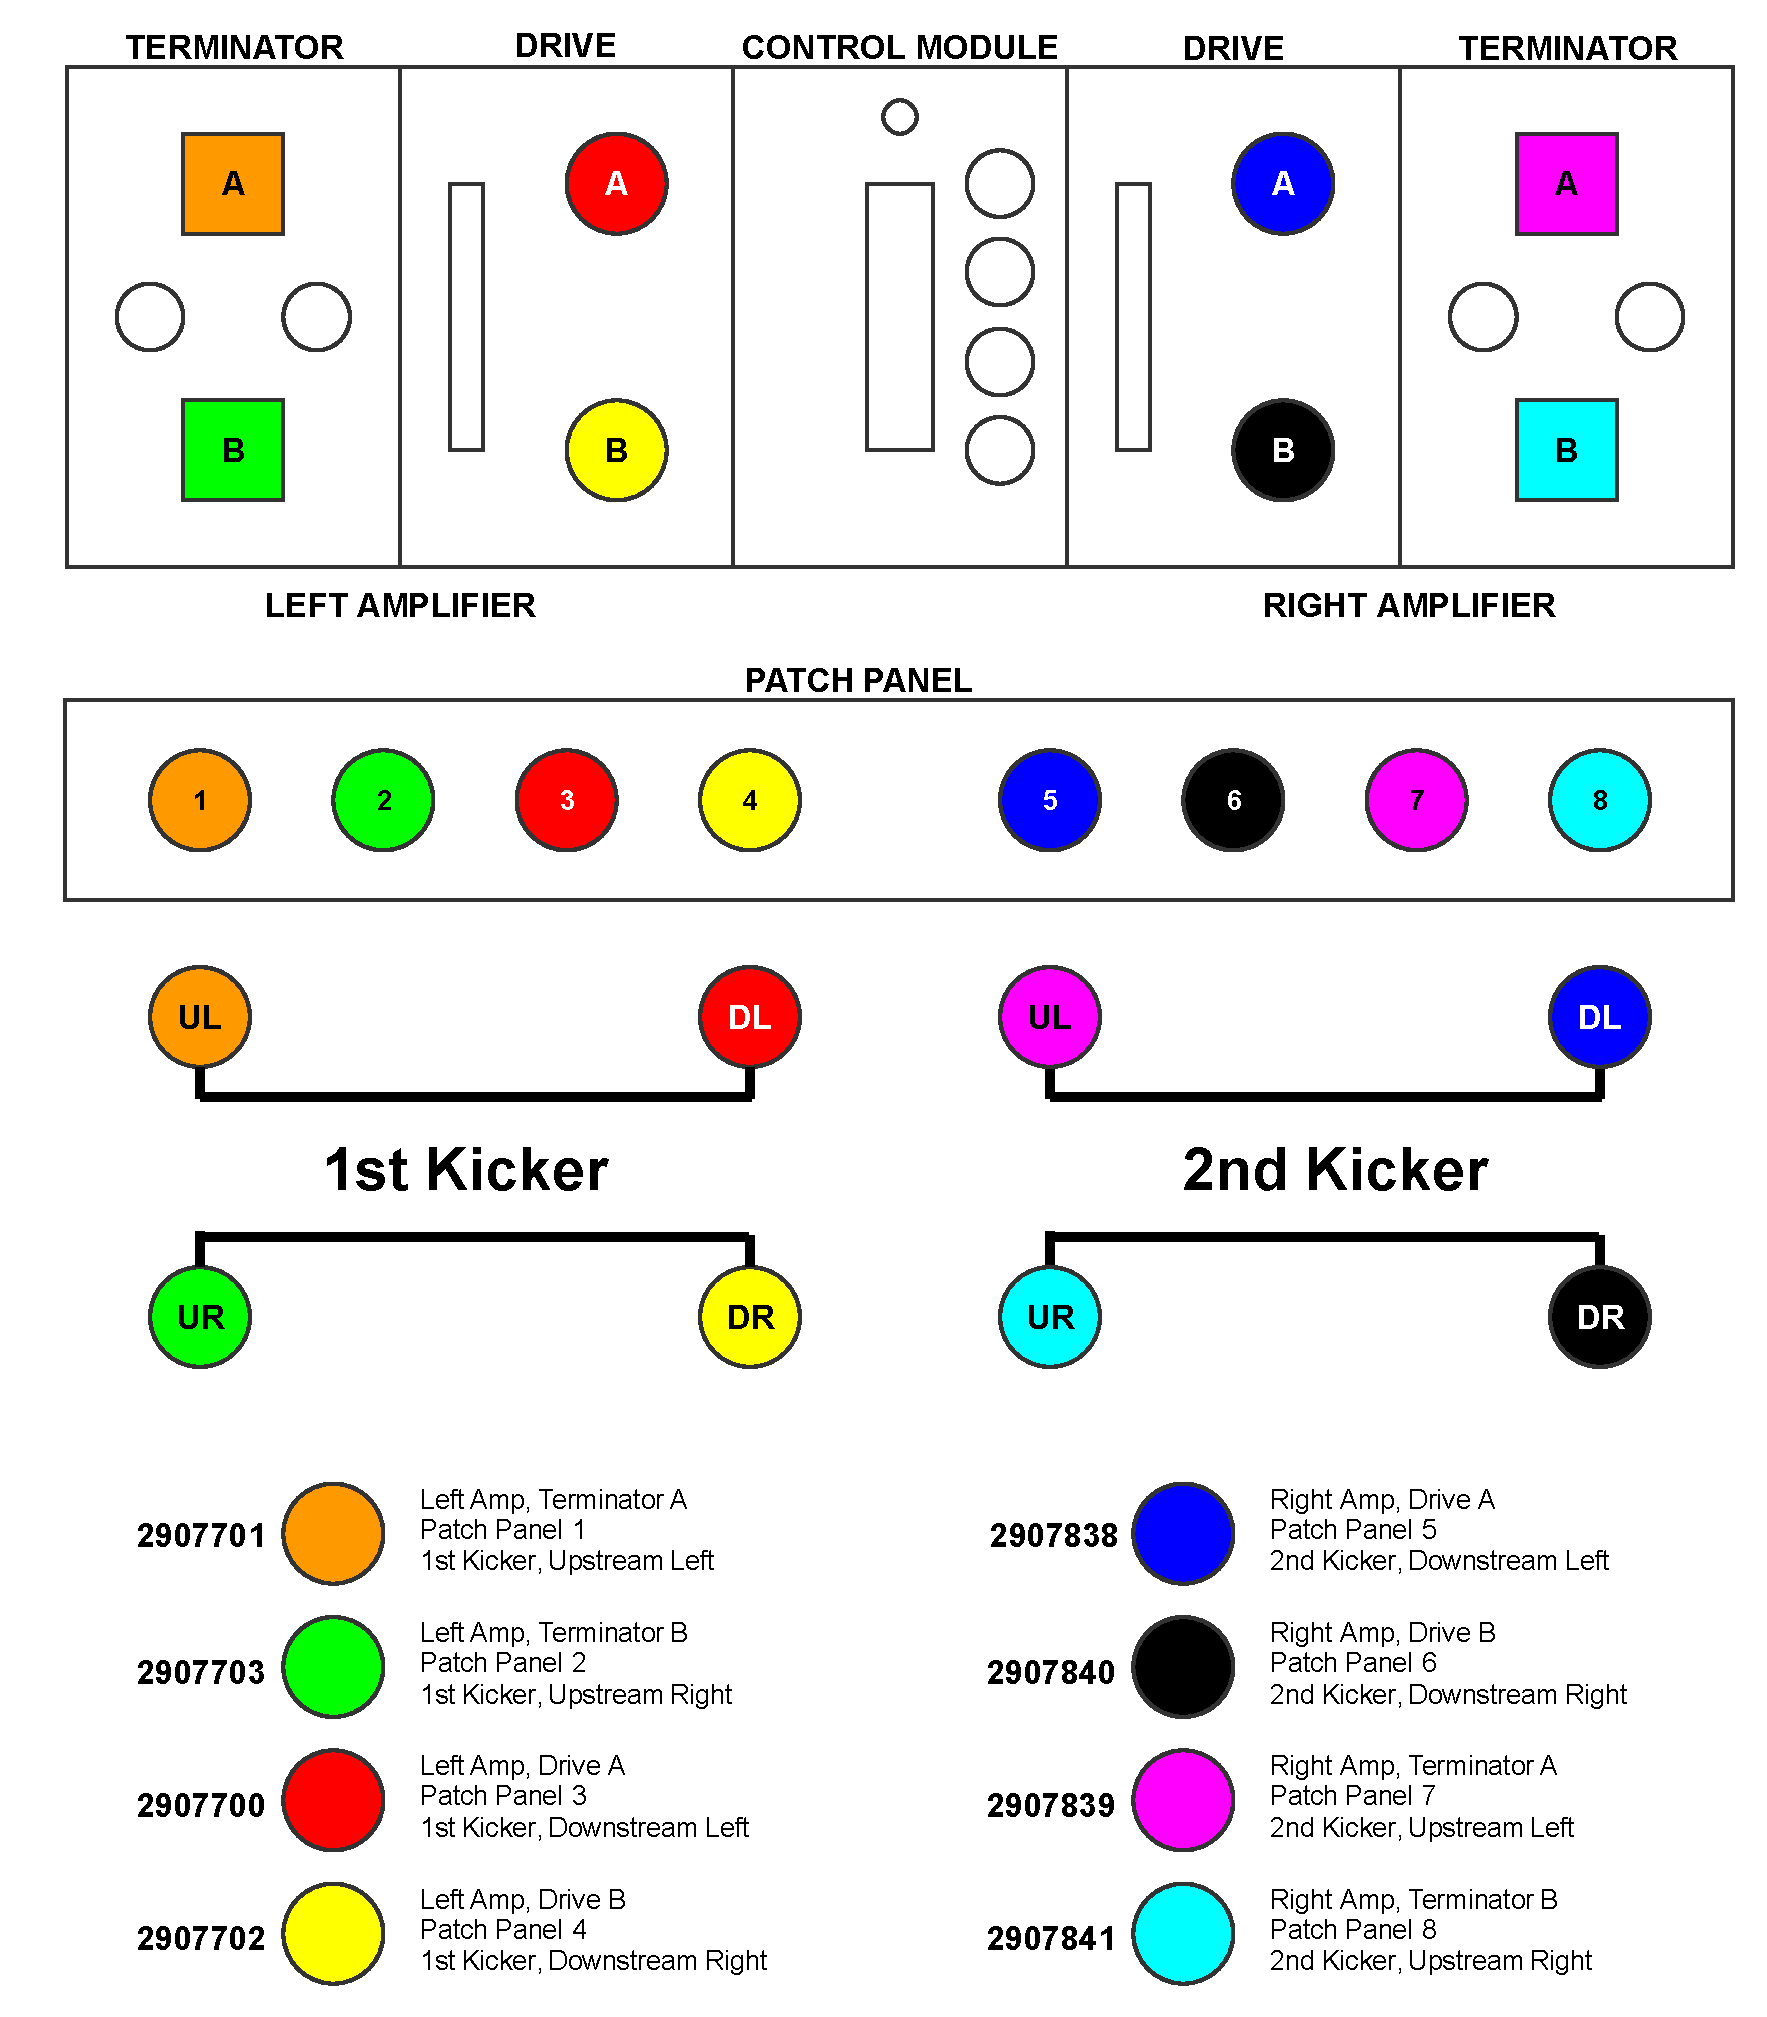
\includegraphics[width=0.9\textwidth]{Figures/commissioning/kickerCables}
  \caption{Cabling setup for cables between the amplifier and kickers.}
  \label{f:kickerCables}
\end{figure}


\subsection{Linearity}
\label{ss:ampLin}

Figure \ref{f:AmpOutvsDAC} shows the amplifier output, as measured by the monitoring signals, at different constant input voltages sent from the FONT5a board between the minimum of -2V (-4096 DAC counts) and maximum of 2V (+4096 DAC counts). The output voltage from the monitoring signals is converted in to the real amplifier output Voltage using the approximate conversion factor of 115. All four amplifier outputs are shown (one for each strip of the two kickers). The plotted values are means taken across a 480~ns central part of the whole 1400~ns output pulse.

The relative polarity of the four outputs is equivalent to what would be sent to the kickers during PFF operation, with opposite polarity of the L and R amplifier outputs sent to each kicker, so that the beam is kicked in opposite directions by each kicker with the second kicker then closing the orbit bump created by the first. Within each side of the amplifier the A and B outputs (sent to each side of the kicker) also have opposite polarity, necessary to create the potential difference across the strips within each kicker that creates the deflecting field for the beam. The relative polarity of the A and B outputs is fixed in the amplifier design and cannot be controlled via the FONT5a board.

The response of the amplifier is highly linear in the region between \(\pm1.2\)~V sent to the amplifier. Outside this range the amplifier clearly begins to enter saturation, in particular above input voltages of \(\pm1.7\)~V. The linear fits shown include only the points between \(\pm1.2\)~V, excluding the first and last three points in the scan of input voltages, in order to not be biased by the effects of saturation.

Figure \ref{f:AmpOutvsDAC_residual} shows the residuals between the linear fit and the real amplifier output across the full range of input voltages. By looking at the residuals a slight deviation from linearity in the \(\pm1.2\)~V range is also visible, although the maximum difference is only 10~V or a 3\% relative error. At the maximum input voltage of \(\pm2\)~V the difference between the real output and the amplitude expected if the response was linear across the full range rises above 150~V, or a relative error of more than 25\%. For example, the RB output at an input voltage of \(+2\)~V is 605~V but the fitted response gives 769~V, a difference of 164~V or 27\%.

The effects of amplifier saturation are not taken in to account in the PFF algorithm on the FONT5a board, in which the DAC output is linearly dependent on the input phase (voltage from the phase monitor mixer signal) across the full range. The applied correction to the downstream phase will therefore be non-optimal when the DAC output calculated by the PFF algorithm is above an absolute value of 2500 counts (1.2~V sent to the amplifier). To date the non-linearity of the amplifier as it begins to enter saturation has also not been included in the PFF simulations presented in the following chapters. This may partially explain the small discrepancies seen between the simulated and real results in some datasets, so including the effect will be pursued in the future. In addition, it could be foreseen to incorporate the saturation characteristics in to the PFF algorithm on the FONT5a board, so that calculated outputs above 2500 counts are boosted slightly to compensate for the lower than expected amplifier output.

Discrepancies between the four amplifier outputs are also visible in Figure~\ref{f:AmpOutvsDAC_residual} and Table~\ref{t:AmpOutVsDAC}, both in terms of gradient and peak output. This can be partially but not completely explained by errors of up to a few percent in the precise calibration of the four monitoring outputs, which do not output exactly 1/115 of the real input voltage [TODO: Ask Colin about errors]. Differences between the A and B outputs sent to each kicker are not an issue for the PFF performance as both are linear (in the \(\pm1.2\)~V range) and the kick experienced by the beam in each kicker is proportional to the difference of the two. Therefore, only the calibration between the output from the FONT5a board sent to the amplifier and the resulting phase shift in the TL2 chicane is affected. However, disparity between the potential difference across each kicker (LA-LB and RA-RB), so that the deflection of the beam in each kicker is different, leads to the orbit bump created by the PFF system not being closed in the chicane, degrading the horizontal beam stability downstream. The fitted potential difference at 1~V input is 869~V for the left amplifier (LA-LB, sent to the first kicker) and 835~V for the right amplifier (RA-RB, sent to the second kicker), a difference of 4\%. This can be compensated in the PFF setup on the FONT5a board by using a different gain for each correction output, so that the voltage sent to the right amplifier is higher but the resulting output voltage sent to both kickers is the same. Orbit closure is discussed further in Section~\ref{ss:orbitClosure}.


\begin{figure}
  \centering
  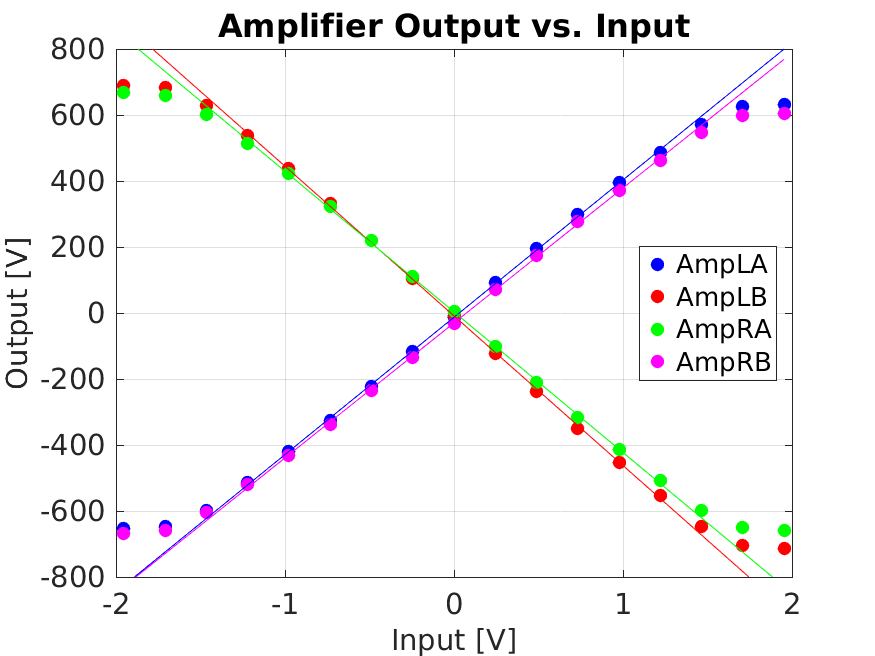
\includegraphics[width=0.9\textwidth]{Figures/commissioning/AmpOutvsDAC}
  \caption{Amplifier output vs. input.}
  \label{f:AmpOutvsDAC}
\end{figure}

\begin{figure}
  \centering
  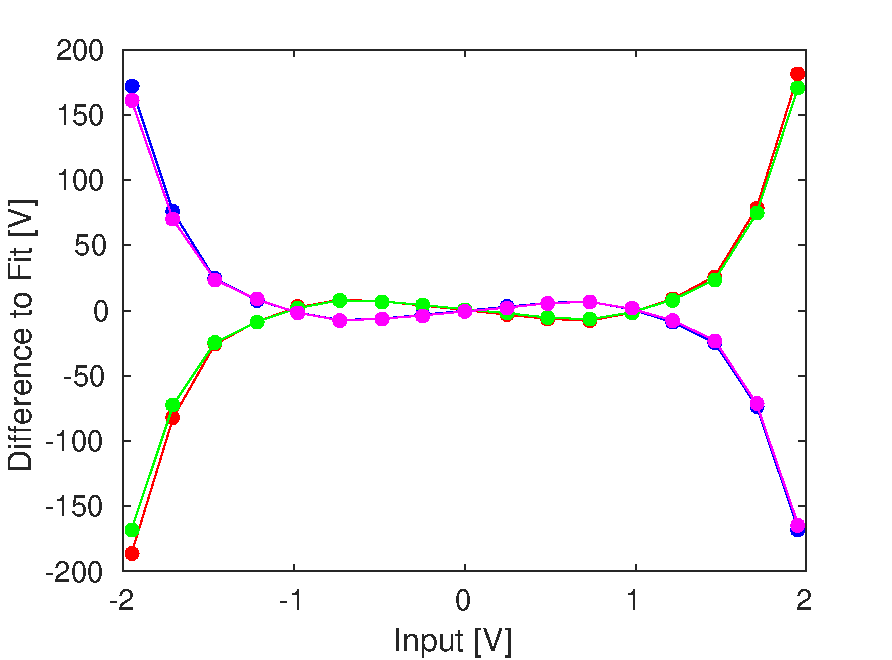
\includegraphics[width=0.9\textwidth]{Figures/commissioning/AmpOutvsDAC_residual}
  \caption{Residual between amplifier output and linear fit.}
  \label{f:AmpOutvsDAC_residual}
\end{figure}

\begin{table}
  \begin{center}
    \begin{tabular}{| c | c |}
	   \hline
       Amplifier Port & Output at +1~V Input \\ \hline
       LA & \(+416\pm3\)~V \\
	   LB & \(-453\pm3\)~V \\
	   RA & \(-426\pm3\)~V \\
	   RB & \(+409\pm3\)~V \\
 	   \hline
    \end{tabular}
    \caption{Feedforward results using combined data from 20th November 2015.}
  	\label{t:AmpOutVsDAC}
  \end{center}
\end{table}

\subsection{Shape}
\label{ss:ampShape}

In the previous section the linearity of the mean output was considered but the performance of the PFF correction is clearly also sensitive to any variations in output voltage along the amplifier output pulse. Figures~\ref{f:ampLTraces} and \ref{f:ampRTraces} show the full 1.4~\(\mathrm{\mu}\)s amplifier output pulse at a constant \(+1\)~V input sent to the left amplifier and a constant \(-1\)~V input sent to the right amplifier respectively. Spikes in the signal just prior to 2000~ns and after 3000~ns on the time axis as seen in the plots are beam pickup induced by the beam passing through the kickers. These are therefore not a property of the amplifier performance and are excluded from the analysis in this section. However, the beam pickup is used later in Section~\ref{ss:absTiming} for the purposes of optimising the correction timing.

\begin{figure}
  \centering
  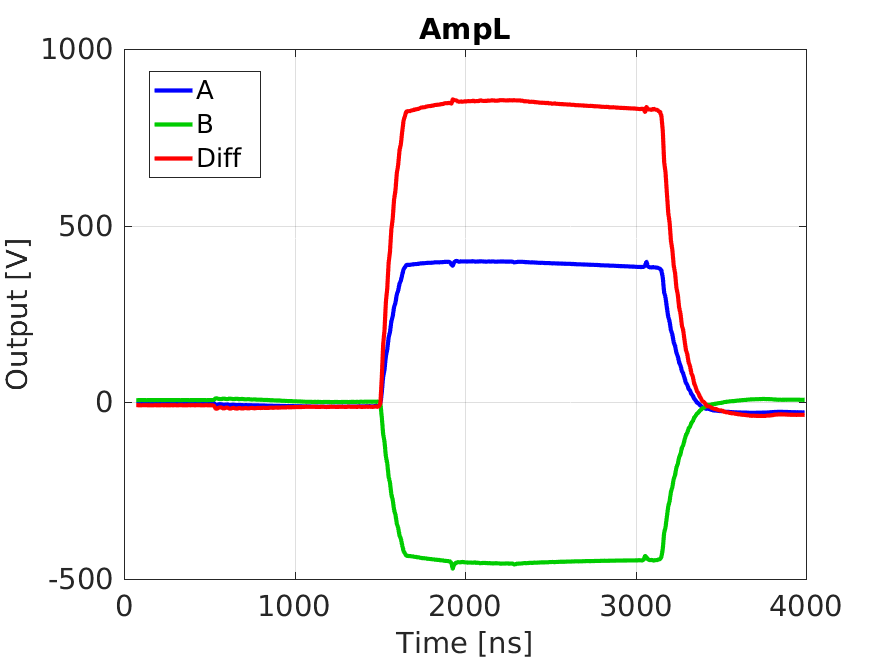
\includegraphics[width=0.9\textwidth]{Figures/commissioning/AmpL_Traces}
  \caption{Amp L along pulse at 1 V input}
  \label{f:ampLTraces}
\end{figure}

\begin{figure}
  \centering
  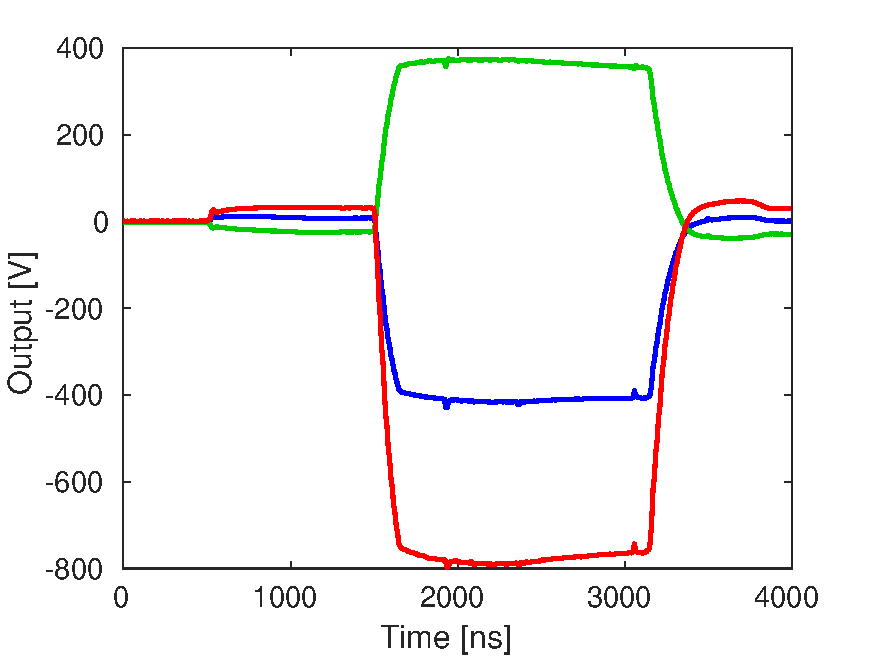
\includegraphics[width=0.9\textwidth]{Figures/commissioning/AmpR_Traces}
  \caption{Amp R along pulse at 1 V input}
  \label{f:ampRTraces}
\end{figure}

For each side of the amplifier both the A and B outputs are plotted as well as the difference of the two, which is the relevant quantity in terms of the kick received by the beam as it traverses the kickers. In the ideal case the potential difference should be flat along the full pulse length. However, for both the left and right side variations in the difference are visible, with an initial increase in output across the first 500~ns of the pulse followed by a droop in response across the second half of the pulse. Although not shown here, the shape of the variations along the pulse is consistent across the full range of output voltages, and scale in magnitude with the output voltage. Figure~\ref{f:ampFlatness} shows the peak-to-peak and mean deviation of the output voltage along the pulse across the full range of input voltages. The peak-to-peak deviation refers to the difference between the minimum and maximum output along the pulse, whilst the mean deviation is the average absolute difference between the mean output and the output at each sample point. For a constant input voltage the output voltage along the pulse varies by up to 88~V peak-to-peak (mean 12~V) for the left amplifier or 93~V peak-to-peak (mean 14~V) for the right amplifier. As a relative difference, this corresponds to approximately a 6~\% peak-to-peak, or 1~\% mean, variation along the pulse.

The PFF algorithm on the FONT5a board uses a single gain value across the whole pulse length for each correction output, thus making the approximation that the amplifier response is flat along the pulse. The variations along the amplifier pulse therefore directly translate in to discrepancies between the intended phase shift as calculated and the real phase shift experienced by the beam. As the region of interest for the correction is a few hundred nanoseconds about the central part of the pulse, as opposed to the full pulse length, the 1~\% mean variation is more indicative of the resulting error than the 6~\% peak-to-peak variation. With a correction range (Section \ref{ss:corrRange}) of \(\pm6^\circ\), the effects of the non-flat amplifier output should be below \(0.06^\circ\) and not measurable considering the phase monitor resolution of \(0.14^\circ\). Nevertheless, it could be foreseen to implement a droop correction in the PFF algorithm on the FONT5a board, taking the variations in the amplifier output along the pulse in to account.

\begin{figure}
  \centering
  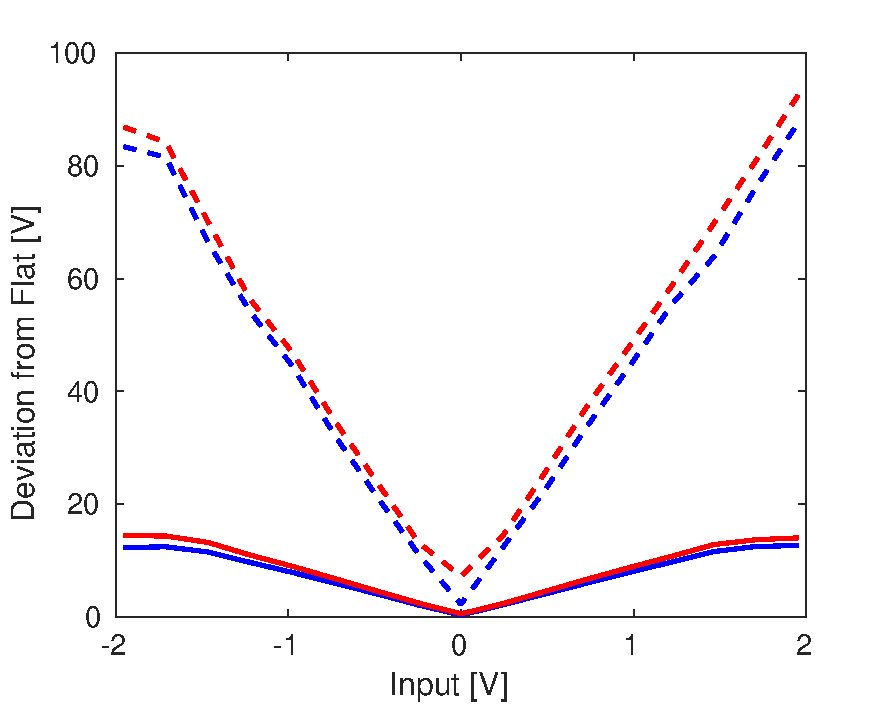
\includegraphics[width=0.9\textwidth]{Figures/commissioning/AmpFlatness}
  \caption{Flatness of potential difference sent to kickers.}
  \label{f:ampFlatness}
\end{figure}

As for the mean output voltage, the second way variations in the amplifier output along the pulse can impact the PFF performance is via the orbit closure in the chicane. For this the relevant quantity is the sum of the potential difference sent to each kicker, or \((LA-LB)+(RA-RB)\). To ensure orbit closure this quantity, named the residual kick here, should be zero across the whole pulse length for all input voltages. Figure \ref{f:ampClosure} shows the residual kick along the pulse for all the input voltages in the scan. Clearly they are not all centred around zero, but this is expected due to the differences in the mean output voltage of the four amplifier outputs seen in the previous section. As already stated, the overall mean offset can be removed by using a different gain for the two correction outputs. However, any variations along the pulse cannot be compensated for in the PFF algorithm. The magnitude of the effect is summarised in Figure \ref{f:ampClosureFlatness}, showing the peak-to-peak and average deviation of the residual kick from flat. The overall residual kick is very flat and effect is smaller than any of those previously shown --- only up to 2~V on the mean or 21~V peak-to-peak. Whether this has any measurable effect on the orbit closure is discussed in Section \ref{ss:orbitClosure}.

\begin{figure}
  \centering
  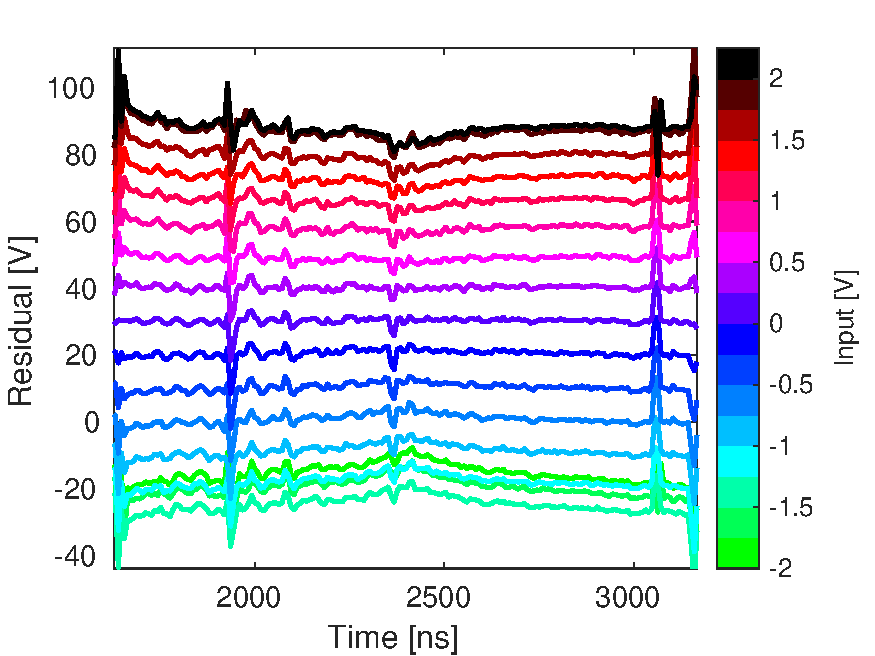
\includegraphics[width=0.9\textwidth]{Figures/commissioning/residualKick_Traces}
  \caption{Residual kick along pulse.}
  \label{f:ampClosure}
\end{figure}

\begin{figure}
  \centering
  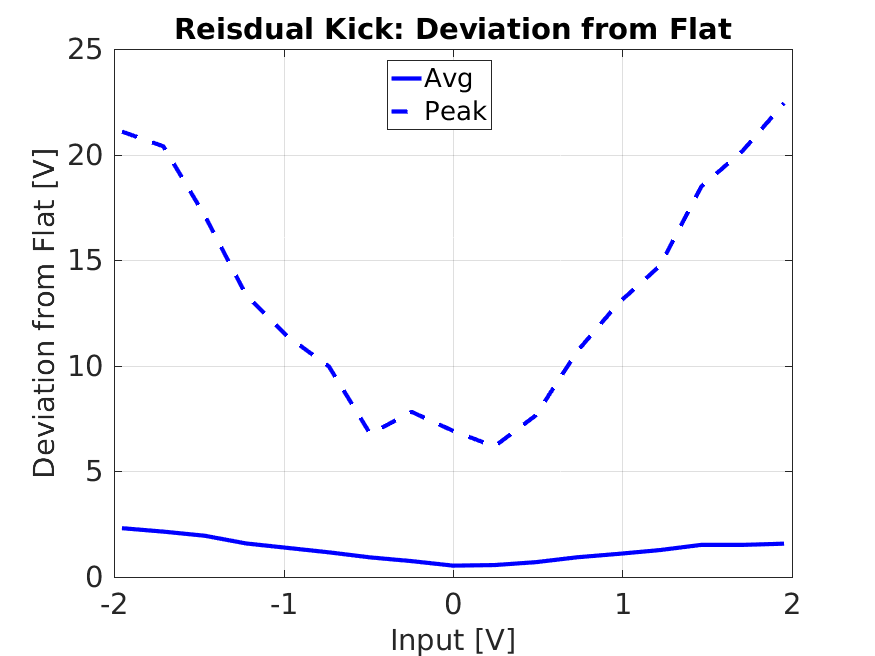
\includegraphics[width=0.9\textwidth]{Figures/commissioning/residualKick_Flatness}
  \caption{Residual kick along pulse: deviation from flat.}
  \label{f:ampClosureFlatness}
\end{figure}

\subsection{Bandwidth}
\label{ss:ampBand}

\newsection{daqSigProc}{Data Acquisition and Signal Processing}

\subsection{SiS Digitiser Setup}
\label{ss:sisSetup}

(already discussed in ph mon chapter)

\subsection{Acquisition Tools}
\label{ss:acqTools}

\subsection{Monitoring Tools}
\label{ss:monTools}

Online display

\subsection{Time Alignment of Signals}
\label{ss:timeAlignment}

\subsection{Definition of Zero Phase}
\label{ss:zeroPhase}



\newsection{constKicks}{Kicker and Optics Performance Verification}

\subsection{Correction Range}
\label{ss:corrRange}

Knowledge of the correction range of the PFF system, or more specifically the relationship between the voltage sent to the amplifier and the phase shift in the chicane, is critical for the PFF setup. The first checks of the ability to shift the phase in the TL2 chicane using the new phase feedforward optics were performed with magnetic correctors prior to the PFF amplifier being available (these correctors can be used to implement a secondary ``Slow Correction'' to complement the PFF system, as discussed in Section~\ref{s:slowCorr}). Aside from their use for the PFF correction, these tests and the clear variation with beam phase versus voltage sent to the PFF kickers shown in this section are already a significant achievement and a verification of the extensive work to improve the MADX model of TL2 presented in Chapter~\ref{c:tl2Optics}. 

Figure \ref{f:phaseVsAmpVoltage} shows the mean phase shift after the chicane (in the downstream phase monitor) across the full \(\pm2\)~V input range of the amplifier. Constant DAC outputs from the FONT5a board were sent to the amplifier in 17 steps between -4096 counts (-2~V) and +4096 counts (+2~V). In order to reduce the sensitivity to any drifts in the beam phase between data points the scan was taken in interleaved mode, alternating between pulses with no drive sent to the amplifier and a constant non-zero DAC output. The phase plotted in Figure \ref{f:phaseVsAmpVoltage} is therefore the difference between 50 kicked beam pulses and 50 ``nominal'' pulses taken at the same time for each amplifier input voltage. 

\begin{figure}
  \centering
  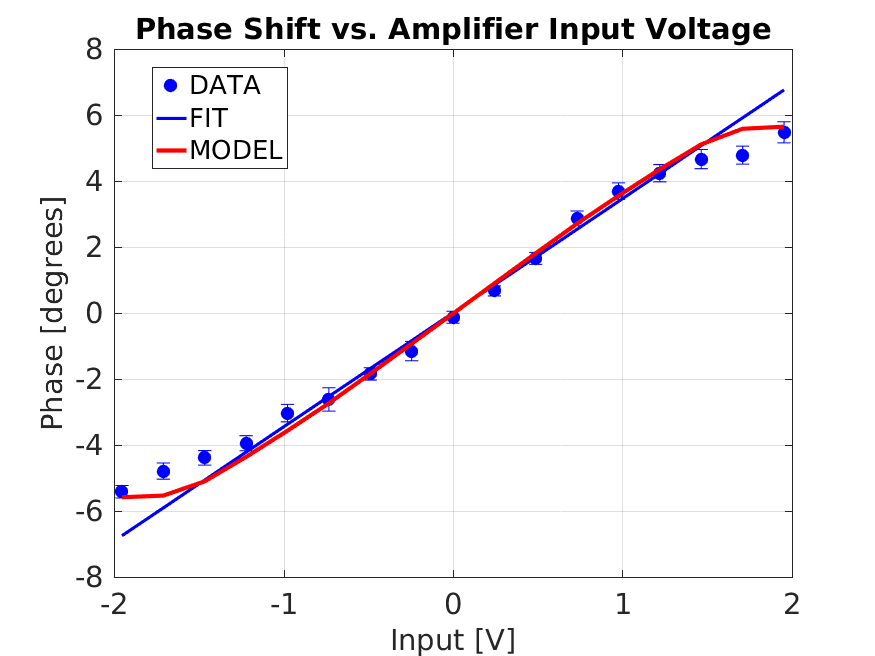
\includegraphics[width=0.9\textwidth]{Figures/commissioning/phaseVsAmpVoltage}
  \caption{Phase shift versus amplifier input voltage.}
  \label{f:phaseVsAmpVoltage}
\end{figure}

\begin{figure}
  \centering
  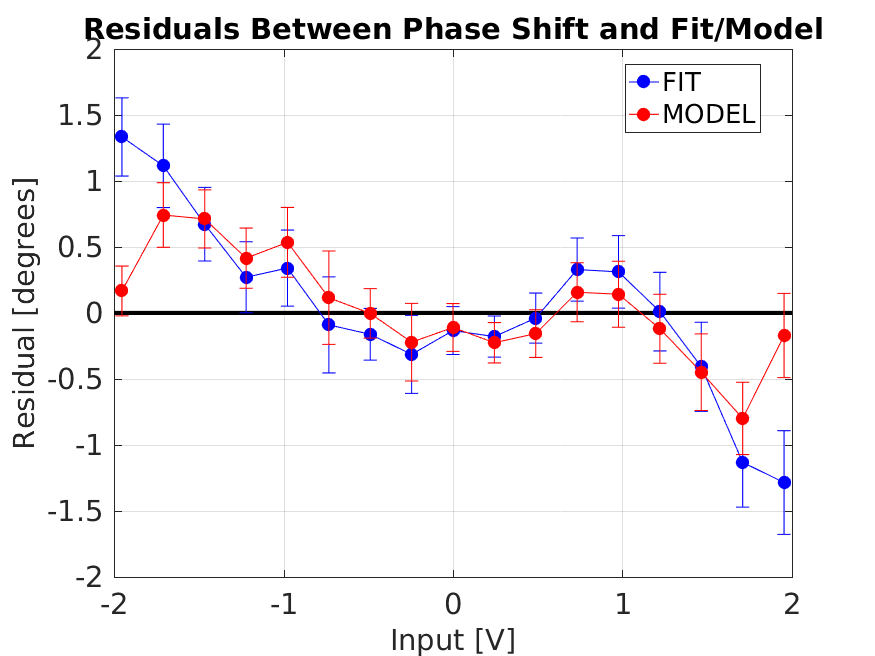
\includegraphics[width=0.9\textwidth]{Figures/commissioning/phaseVsAmpVoltage_residuals}
  \caption{Phase shift versus amplifier input voltage.}
  \label{f:phaseVsAmp_resid}
\end{figure}

\begin{table}
  \begin{center}
    \begin{tabular}{| c | c | c |}
	   \hline
        & Phase Shift at +1~V Input & Max Phase Shift \\ \hline
       Data & \(3.5\pm0.1^\circ\) & \(5.5\pm0.3^\circ\) \\
	   Model & \(3.6^\circ\) & \(5.6^\circ\) \\
 	   \hline
    \end{tabular}
    \caption{Phase shift at +1 volt input to the amplifier.}
  	\label{t:PhaseVsDAC}
  \end{center}
\end{table}

At the maximum amplifier input voltage of \(2\)~V the phase after the chicane is shifted by \(5.5\pm0.3^\circ\). The fitted phase shift per Volt sent to the amplifier is \(3.5\pm0.1^\circ\) in the \(\pm1.2\)~V linear range of the amplifier (excluding the first and last three points, blue ``FIT'' line in Figure~\ref{f:phaseVsAmpVoltage}). This fitted gradient is required and was previously introduced for the conversion between the PFF gain in the units on the FONT5a board and the real applied gain in Section~\ref{ss:pffFirmware}. In Section~\ref{ss:pffFirmware} it was quoted in terms of the phase shift in radians per DAC count output from the FONT5a board, rather than degrees per Volt as shown here. The value of \(30\mathrm{\mu rad/count}\) is easily derived using the conversion factors between degrees and radians and knowing that a DAC output of 4096 counts corresponds to 2~V sent to the amplifier.
[TODO: Calculated factor is 29.827 microradians/count here. One I actually used for gain conversion, simulations etc. was 26.18 (used full range rather than linear range)]

Given knowledge of the amplifier output characteristics (Section~\ref{ss:ampLin}), the kicker specifications (Section~\ref{ss:kickers}) and the chicane optics (Section~\ref{ss:pffMatched}) the real phase shift seen in the scan can be compared to the expected phase shift based on the system parameters. The predicted phase shift, \(\Delta\phi\), in degrees is given by:
\begin{equation}
 	\Delta\phi = V_{amp}[V_{font}].K.R_{52}.\frac{360}{\lambda_{12\mathrm{GHz}}}
\end{equation} 
\label{e:ampVoltToPhase}
Where \(V_{amp}[V_{font}]\) is the amplifier output Voltage at an input voltage of \(V_{font}\) sent from the FONT5a board, \(K\) is the angular deflection of the beam per Volt applied to each kicker strip, \(R_{52}\) is the \(R_{52}\) value between the kickers in the PFF optics and \(\frac{360}{\lambda_{12\mathrm{GHz}}}\) converts the calculated orbit length difference in to an equivalent 12~GHz phase using the 12~GHz wavelength \(\lambda_{12\mathrm{GHz}}\). The value of most of these parameters has already been derived in the sections previously mentioned. They are:
\begin{eqnarray*}
V_{amp}[1~\mathrm{V}] = 435~\mathrm{V} \\
K = 0.8~\mathrm{\mu rad/V}\\
R_{52} = -0.7~\mathrm{m}\\
\lambda_{12\mathrm{GHz}} = 2.5~\mathrm{cm} 
\end{eqnarray*}
The value of \(V_{amp}[1~\mathrm{V}]\) is given as a representative value in the linear range of the amplifier but the real amplifier output at all input voltages is used in the predictions to include the effects of saturation in the calculated phase shift values. Also, the output sent to the first kicker (from the left side of the amplifier) is used as this is most relevant for the phase shift in the chicane (the orbit should be closed after the second kicker with no further phase shift in the chicane after that point). The value of \(K\) is derived from the kicker design, in which 1.4~kV applied to each strip gives a 1~mrad kick for a 150~MeV beam [TODO: REF].  The actual CTF3 beam energy at this time was approximately 135~MeV (calculated based on the dipole currents used in the machine setup), so the value of \(K\) above is scaled by a factor 150/135.

In Figure~\ref{f:phaseVsAmpVoltage} the red line ``MODEL'' shows the predicted phase shifts using Equation~\ref{e:ampVoltToPhase}. Table~\ref{t:PhaseVsDAC} compares the fitted gradients and maximum phase shift for the model and real data. The overall agreement between the two is good, with the residuals between both the model and the data, as well as the linear fit to the data and the data, generally consistent with zero within error bars in the \(\pm1.2\)~V linear range of the amplifier as shown in Figure~\ref{f:phaseVsAmp_resid}. 

Outside the linear range some discrepancies appear, although at the maximum \(\pm2\)~V output the agreement is good so the effect is largest where the amplifier is entering saturation but before hard saturation is reached. However, most amplifier effects can be excluded as the analysis in this section uses the same dataset that was used to characterise the amplifier performance in Section~\ref{s:amplifierSetup}. This could hint at possible remaining higher order errors in the TL2 chicane optics, or unexpected behaviour from the kickers or amplifier. Although subtracting alternating, interleaved pulses should remove the sensitivity to drifts in the machine it is possible that some residual effect remains. To determine whether the discrepancies are reproducible further scans of this type will need to be completed in the future. The residuals between between the data and the linear fit between \(\pm1.2\)~V would also be of significance for the PFF correction should they not converge to zero with additional measurements, as they are of similar magnitude to the \(0.2^\circ\) downstream jitter target. 

However, the overall conclusion is as expected --- the phase shift in the chicane linearly depends on the amplifier input in the \(\pm1.2\)~V (\(\pm2500\) DAC counts) region thus a close to optimal correction can be applied in this range, corresponding to a \(\pm4.2\pm0.1^\circ\) phase shift. However, when the calculated optimal correction is between an absolute input voltage of 1.2~V and 2.0~V, 2500 to 4096 DAC counts, or \(\pm4.2\pm0.1^\circ\) to \(\pm7.0\pm0.2^\circ\), the actual phase shift in the chicane is lower, only up to \(\pm5.5\pm0.3^\circ\), due to the amplifier entering saturation (and possibly other effects to be determined ). Any calculated correction outside \(\pm5.5\pm0.3^\circ\) receives a static phase shift of \(\pm5.5\pm0.3^\circ\) in the chicane. In the limit where all pulses are outside this range the PFF system can only induce a static shift in the mean phase and makes no improvement to the phase jitter. Understanding the impact of the limited correction range on the PFF results was particularly critical for interpreting the early correction attempts with the first version of the amplifier, giving approximately half the ranges shown in this section. This is discussed using simulations of the PFF system in Chapters~\ref{c:earlyFFSim} and \ref{c:feedforward}.

http://accelconf.web.cern.ch/accelconf/ipac2011/papers/tupc007.pdf
1.4 kV to each strip = 1 mrad kick at 150 MeV
1.26 kV to each strip = 1 mrad kick at 135 MeV

\subsection{Variations Along Pulse}
\label{ss:kickPulseVar}

In this section I intended to check the stability of the constant kick along the pulse, as I did for the "Shape" section with the amplifier above. The results from the constant kick data do not look good, though - the errors are quite large and there are some nasty oscillations along the pulse, such as in the example Figure~\ref{f:phaseShiftAlongConstKick}. With the phase stability downstream a much longer scan would probably be needed to draw conclusions here, though even on longer time scales I think it needs to be checked that the difference between odd and even pulses converges to zero. As it is I would probably choose to skip this section, or possibly just show one of the better plots.

\begin{figure}
  \centering
  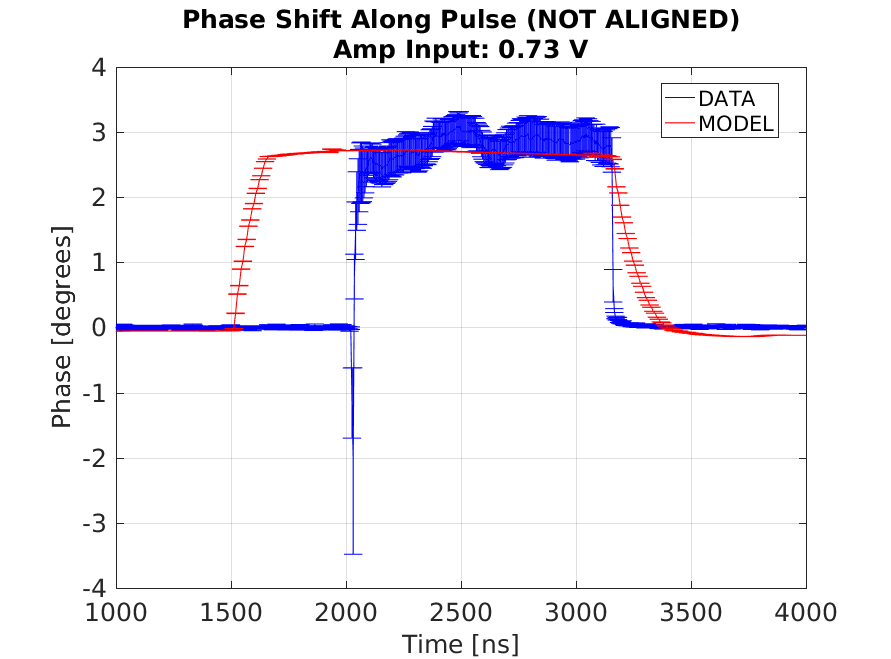
\includegraphics[width=0.9\textwidth]{Figures/commissioning/phaseShiftAlong}
  \caption{Traces relative timing scan.}
  \label{f:phaseShiftAlongConstKick}
\end{figure}

\subsection{Shape}
\label{ss:kickShape}

The purpose of this section is to compare the shape of the given kick to the upstream phase - i.e. compare the upstream phase to the amplifier monitoring output and the difference in the downstream phase with PFF off and on. Again here my first attempts produced results that were not as I'd like, without particularly good agreement between the difference in the downstream phase and the upstream phase shape. Looks kind of like the two are rotated with respect to each other. More analysis needed here to check more thoroughly. I think this section should definitely be included, but I need either an explanation for the differences or to find datasets where the agreement is much better.

\begin{figure}
  \centering
  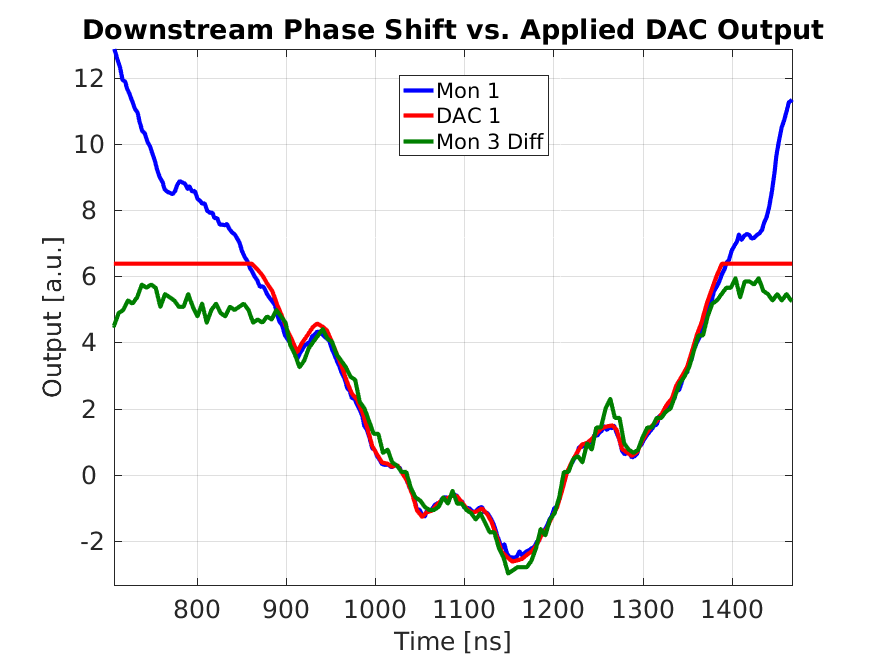
\includegraphics[width=0.9\textwidth]{Figures/commissioning/pffKickShape}
  \caption{Traces relative timing scan.}
  \label{f:pffKickShape}
\end{figure}

\subsection{Orbit Closure}
\label{ss:orbitClosure}

At CLIC the PFF system must not degrade the transverse beam stability. This means for any voltage sent to the kickers the horizontal beam orbit after the PFF chicane must be unchanged, or closed, despite the different orbits inside the chicane. As such, the PFF optics for the TL2 chicane at CTF3 is also designed to give a closed kick, as presented in Section~\ref{ss:pffMatched}. However, up until now the main focus during PFF operation has been the primary goal of reducing the downstream phase jitter and ensuring good beam transmission to the downstream phase monitor. As a result orbit closure after the TL2 chicane has not yet been strictly enforced during PFF operation as will be seen in this section, but the current status is shown here as an additional cross-check of the PFF optics and to highlight where improvements are needed for future tests.

Using the same constant kick data as Section~\ref{ss:corrRange} Figure~\ref{f:HOrbitVsInput} shows mean the horizontal orbit before, inside and after the TL2 chicane across the full \(\pm2\)~V range of inputs sent to the amplifier. The vertical black lines on the plot mark the approximate location of the entry to the chicane (index CC.500) and the exit of the chicane (index CC.800), with the two kickers being located at CC.480 and CC.780. Two BPMs before and after the chicane, as well as the four inside the chicane, are included. The plotted positions are the difference between the kicked and nominal (non-kicked) orbit at each BPM, thus removing any misalignment in the BPM centres. Before the chicane and the first kickers there is no significant effect on the orbit as expected. Inside the chicane the PFF system induces an orbit offset of up to \(1.4\pm0.1\)~mm. After the chicane, in BPMs CC.845 and CC.930, the orbit should return to zero in the ideal case. However, a clear residual offset can be seen, up to \(0.5\pm0.1\)~mm in CC.930.

\begin{figure}
  \centering
  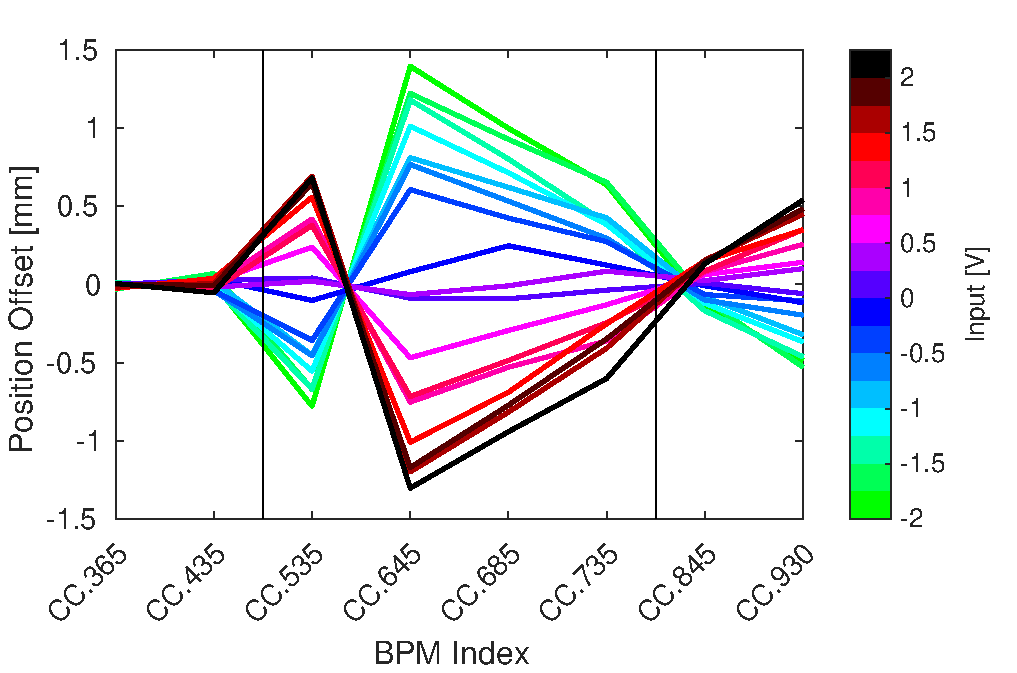
\includegraphics[width=0.9\textwidth]{Figures/commissioning/HOrbitVsInput}
  \caption{Horizontal orbit offset in and around the TL2 chicane at different input voltages sent to the amplifier.}
  \label{f:HOrbitVsInput}
\end{figure}

During this scan the input sent to both sides of the amplifier was the same magnitude. However, in Section~\ref{ss:ampLin} it was seen that the right side of the amplifier, sent to the second kicker, gave 4\% lower output than the left side. This could explain why the orbit after the chicane was not closed during this scan, and during PFF operation which has typically used equal gain for both correction outputs to date. Figure~\ref{f:orbClosureVsAmpModel} shows the expected orbit in the TL2 chicane in the case where both kickers are driven with the same voltage (``nominal optics'') and with the 2nd driven with a 4\% lower voltage (``real amplifier ratio'').
\footnote{The term ``nominal optics" is used in this section to refer to the nominal PFF optics, not the nominal optics created in Chapter~\ref{c:tl2Optics} to use when the PFF system is not under operation.}
The full MADX orbit propagated through all elements is shown, with the eight real measured BPM offsets also included at their respective positions. Each BPM point represents the gradient of a linear fit using the variation with input voltage seen previously in Figure~\ref{f:HOrbitVsInput}. Before and inside the chicane the agreement between the BPM data and the model is excellent. As seen before, the BPM orbit is not closed after the chicane, unlike the nominal optics. If the actual kicker voltage ratio is taken in to account the MADX orbit after the chicane is not closed either, but the offset has opposite polarity to the real data in the last BPM.

\begin{figure}
  \centering
  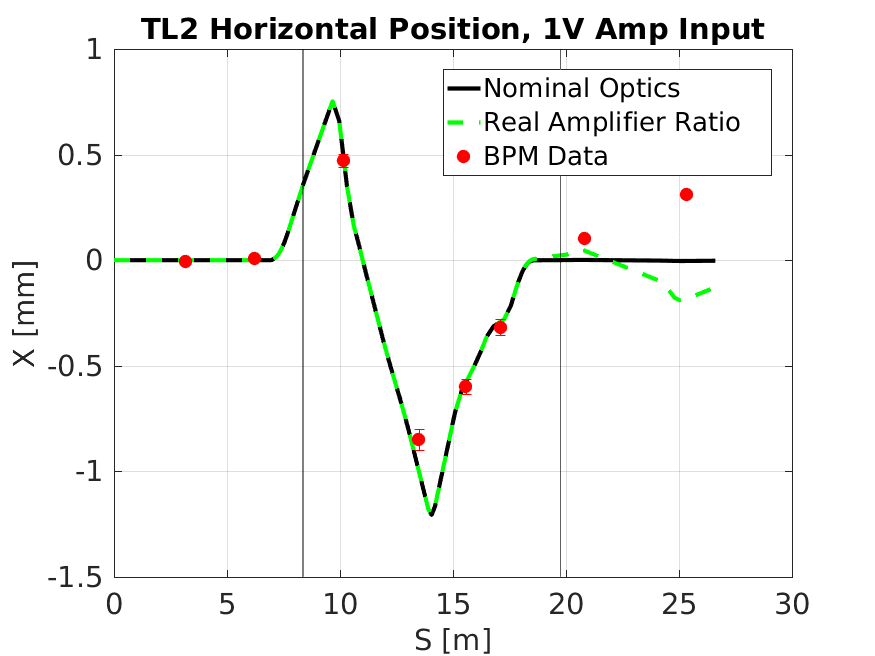
\includegraphics[width=0.9\textwidth]{Figures/commissioning/orbClosureVsAmpModel}
  \caption{Orbit in the TL2 chicane at 1~V amplifier input for the BPM data, nominal model and model taking in to account the difference in amplifier output voltage to each kicker.}
  \label{f:orbClosureVsAmpModel}
\end{figure}

The true explanation for the non-closed orbit is that the quadrupole strengths used in the machine setup are not exactly nominal. Although every effort has been made to keep the TL2 optics as close to nominal as possible, particularly inside the chicane, it is an extremely sensitive area for the setup of CTF3 and beam transport in to the CLEX area downstream of TL2 (including the location of the downstream phase monitor in the TBL line) is always difficult. Minor modifications have therefore been necessary in order to achieve full beam transmission to the downstream area, both for PFF and other experiments at CTF3. The largest changes have been made to the four quadrupoles following the chicane but one quadrupole inside the chicane, CC.IQFL0730 (just prior to the 2nd kicker) has a set value \(10\%\) lower than the nominal optics, as well as differences up to \(2\%\) in the other quadrupoles. Using the real quadrupole strengths used in the machine gives the result shown in Figure \ref{f:orbClosureVsQuadModel}. In this case the agreement between the model and the data is also extremely good after the chicane. It may still be possible to compensate for these differences by outputting different voltages to each kicker and this will be investigated. Alternatively, a completely nominal optics can be set in the chicane purely for the purposes of verifying orbit closure, reverting back to non-nominal optics and closure if needed to achieve good beam transmission for normal PFF operation.

[TODO: Not enough detail r.e. why beam transport there is difficult etc.?]

[TODO: Do have data with different ratios of kicker strengths. Can analyse to see effect on closure. Considering quad currents don't think it adds anything to discussion here, though.]

\begin{figure}
  \centering
  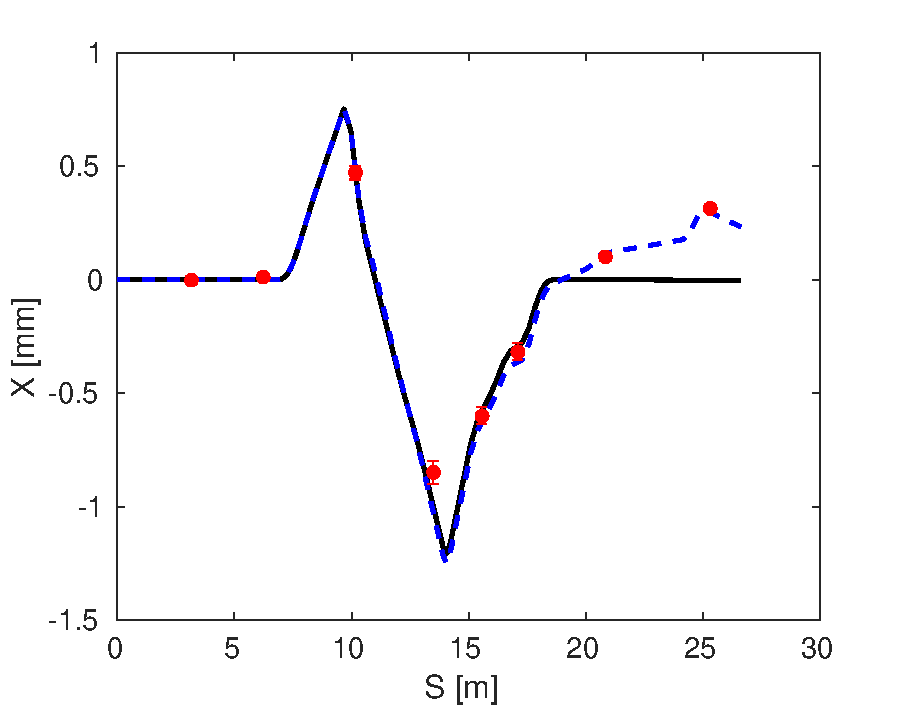
\includegraphics[width=0.9\textwidth]{Figures/commissioning/orbClosureVsQuadModel}
  \caption{Orbit in the TL2 chicane at 1~V amplifier input for the BPM data, nominal model and model taking in to account the quadrupole currents in the real machine setup.}
  \label{f:orbClosureVsQuadModel}
\end{figure}

[Comment for Piotr: With these quad currents also expect to see some dispersion leaking  out of the chicane. Up to 0.3 m in girder 9.]

\newsection{timing}{Correction Output Timing}

\subsection{Kicker Cable Lengths}
\label{ss:kickerCables}

Kicker why drive downstream end theory
Cable length measurements (tdr, matching length of drive pairs)




\subsection{Absolute Timing}
\label{ss:absTiming}



\subsubsection{Using Beam Pickup}
\label{sss:beamPickup}

[TODO: Kicker pick-up theory. In particular, is time between pickup exactly the beam pulse length or is it longer by double the kicker length?]

Figure~\ref{f:beamPickup_noKick} shows the beam pickup at the start and end of the pulse from the PFF kickers at CTF3, as seen on one of the amplifier monitoring outputs (each of the four amplifier monitoring outputs, one for the upstream end of each strip prior to the signal being terminated at the amplifier, gives a similar response). The separation of the peaks in the beam pickup is \(1.1~\mathrm{\mu s}\), thus the same as the CTF3 pulse length as expected. By comparing the timing of these peaks with respect to the start and end of the amplifier output pulse, using the same amplifier monitoring signal, it is possible to ensure that the correction output arrives in sync with the beam.

\begin{figure}
  \centering
  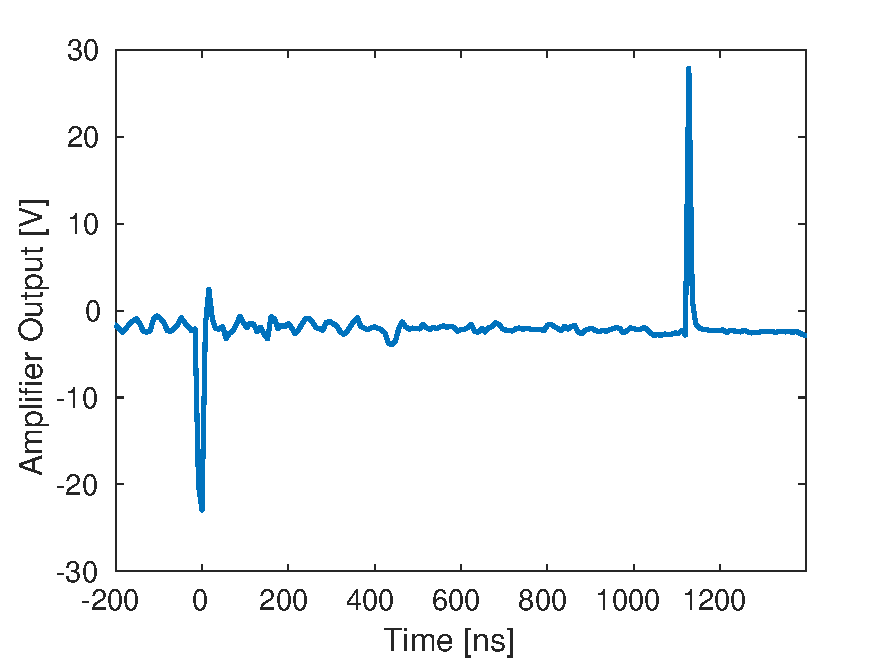
\includegraphics[width=0.9\textwidth]{Figures/commissioning/beamPickup_noKick}
  \caption{Beam pickup on kicker strips as seen on amplifier monitoring signals.}
  \label{f:beamPickup_noKick}
\end{figure}

An example of this is shown in Figure~\ref{f:absDelay0_all}. A constant DAC output is sent from the FONT5a board to the amplifier and both this output pulse and the beam pickup, at samples 275 and 493, are visible in the figure. Importantly, the DAC output is gated using the upstream phase monitor diode signal (in other words, the constant DAC output is only sent during the time when the diode is non-zero) and this has two consequences. Firstly, the amplifier output pulse has the same length as the beam pulse in the upstream phase monitor. Secondly, the timing of the output is identical to what it would be in normal PFF operation. In the case of Figure~\ref{f:absDelay0_all} the drive to the amplifier is sent as quickly as possible after the arrival of the upstream diode signal at the FONT5a board. It can be seen that the amplifier pulse arrives before the beam pickup, thus with the PFF system setup this way the correction would be applied slightly early. This result therefore proves that the PFF system just meets the latency requirements, with the overall time needed to transport and process all the relevant signals a few tens of nanoseconds less than the 380~ns time of flight of the beam between the upstream phase monitor and the first kicker. However, what is also clear in the figure is that the time offset between the start of the amplifier pulse and the first beam pickup spike is much larger than the time difference between the end of the amplifier pulse and the second beam pickup spike. This is due to the energy transient across the first 100~ns of the CTF3 beam pulse which is present in the upstream phase monitor but is then lost prior to the TL2 chicane, predominantly in TL1. As a result the downstream beam pulse is shorter than the upstream beam pulse which defines the length of the correction output. Therefore, in order to align the correction output with the beam the signals from the end of the amplifier and beam pulses must be used, not the start.

\begin{figure}
  \centering
  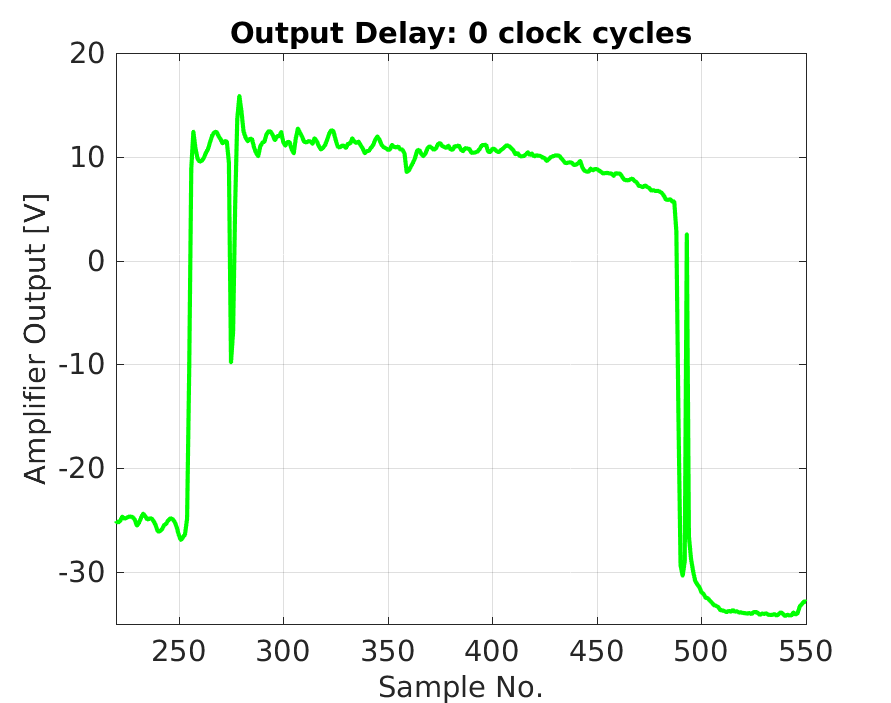
\includegraphics[width=0.9\textwidth]{Figures/commissioning/absDelay0_all}
  \caption{Output delay of 0 clock cycles. Full pulse.}
  \label{f:absDelay0_all}
\end{figure}

The firmware for the FONT5a board includes an output delay parameter that can be used to fine-tune the timing of the correction output sent to the amplifier. This can be done independently for each of the two correction outputs so that it can be ensured the correction arrives in sync with the beam in each kicker individually (the relative timing of the two kickers is discussed in the next section). The delay can be varied between 0~and~31~clock~cycles in integer steps, with one clock cycle corresponding to one period of the 357~MHz ADC clock frequency, or 2.8~ns. A delay of up to 86.8~ns can therefore be added to the correction outputs. Figure~\ref{f:absDelayAll_endPulse} shows the effect of varying the output delay across the full range of possible values, zoomed in on the end of the pulse. For all output delays the beam pickup remains at sample 493, as expected. Meanwhile, the end of the amplifier pulse is moved from before the beam pickup (output too early) to after the beam pickup (output too late). To achieve the optimal correction timing the end of the amplifier pulse must be aligned with the beam pickup and this is achieved with a delay of 7~clock~cycles, or 19.6~ns, as shown in Figures~\ref{f:absDelay7_all}~and~\ref{f:absDelay7_end}. This delay has been used for the latest PFF runs presented in Chapter~\ref{c:feedforward}. Due to ambiguity in which point along the falling edge of the amplifier pulse the beam pickup should be aligned to there may be a remaining error of up 3 clock cycles in the exact alignment, and this can only be verified by beam based measurements (not using the amplifier monitoring outputs). 

\begin{figure}
  \centering
  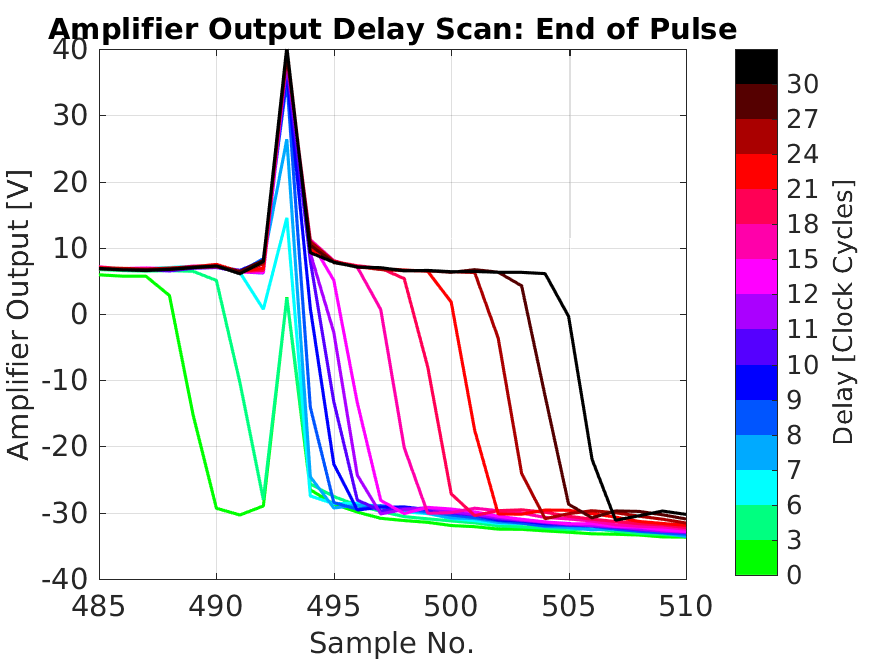
\includegraphics[width=0.9\textwidth]{Figures/commissioning/absDelayAll_endPulse}
  \caption{Output delay scan, end of pulse.}
  \label{f:absDelayAll_endPulse}
\end{figure}

\begin{figure}
  \centering
  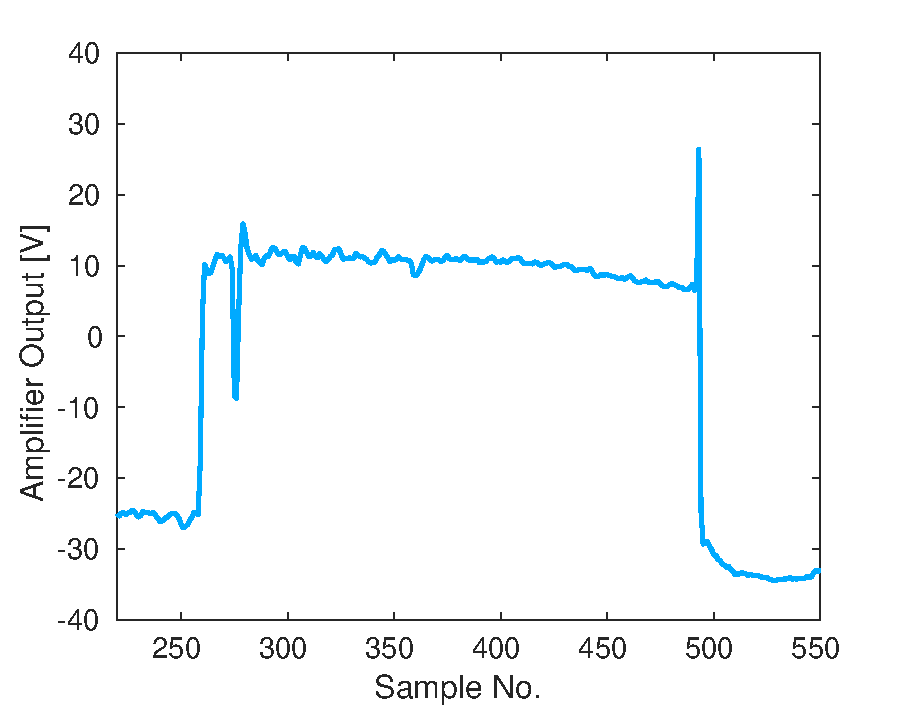
\includegraphics[width=0.9\textwidth]{Figures/commissioning/absDelay7_all}
  \caption{Output delay of 7 clock cycles. Full pulse.}
  \label{f:absDelay7_all}
\end{figure}

\begin{figure}
  \centering
  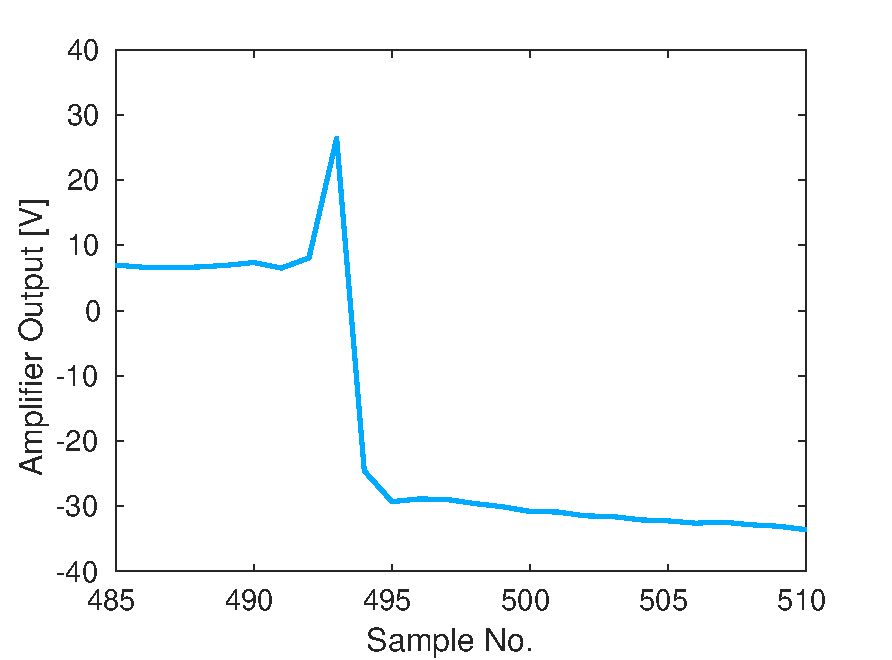
\includegraphics[width=0.9\textwidth]{Figures/commissioning/absDelay7_end}
  \caption{Output delay of 7 clock cycles. End of pulse.}
  \label{f:absDelay7_end}
\end{figure}


\subsubsection{Using BPMs}
\label{sss:relativeBPM}

This section presents one way in which the correction output timing can be determined using a combination of the phase monitor measurements and a BPM signal downstream of the TL2 chicane. The results shown here were performed with the first, lower power version of the amplifier and the FONT5 rather than the later FONT5a board, and because of this the optimal output delay calculated here does not agree with the value of 7~clock~cycles from the beam pickup based measurement above. The newer hardware has the same latency as the previous versions, thus the difference does not come from hardware changes but rather associated changes to cabling between the phase monitor electronics, FONT5a board and amplifier. The measurement will be repeated in the future to verify that both methods give consistent results when the same hardware and cabling setup is used.

The FONT5 (and FONT5a) board firmware provides the functionality to be able to change the gain of each PFF correction output independently. This means it is possible to apply the correction to only one kicker, or to kick the beam in the same direction in each kicker (i.e. to use the same sign for the gain in each kicker, rather than gains with equal magnitude but opposite sign). In both of these cases the kicked PFF orbit in the chicane is not closed, thus the horizontal position along the beam pulse in a BPM after the chicane depends on the shape and timing of the applied correction.\footnote{In Section~\ref{ss:orbitClosure} it was shown that the corrected orbit is not perfectly closed in normal PFF operation either. However, in this case no attempt at orbit closure is made so the measured effect seen in the BPMs is much larger.}

Figure~\ref{f:absTimBeam_d0} compares the upstream phase, downstream phase and horizontal position (in a BPM after the TL2 chicane) along the pulse in the case where the PFF correction is applied with gains set to kick the beam in the same direction in each kicker, and with no output delay applied in the FONT5 board. The data is taken in interleaved mode, with the plotted phases shown using the PFF off data and the BPM trace being the difference between the PFF on and PFF off data. Each signal is scaled and sign flipped where necessary to give variations along the pulse with the same magnitude and sign, in arbitrary units. The BPM and phase monitor signals are acquired with the same sampling frequency of 192~MHz, with each aligned so that the end of the pulse is at the same sample number. 

By taking the difference of the PFF off and PFF on data in the BPM any residual orbit variations along the pulse not related to the PFF system are removed, thus the remaining shape should match that of the PFF correction output, which in turn is linked to the upstream phase. The downstream phase should also have the same shape as the upstream phase with the PFF system off, within the limits of the upstream-downstream phase correlation achieved at this time. During this measurement many oscillations along the upstream phase were present, which usually are not desired but for this measurement are perfect points of reference to check the time alignment of the signals. As expected the overall shape of the residual horizontal position in the BPM along the pulse and the two phase signals is very similar. The largest feature in the upstream phase that is present in all three signals occurs at sample 671 in the upstream phase, with the location of the peak of this oscillation in the phase signals and the BPM marked by vertical black lines in the figure. The peak as seen in the BPM signal is clearly before the peak in the phase monitor signals thus in this case the correction was applied early, with a measured offest of -36~ns between the peaks.

\begin{figure}
  \centering
  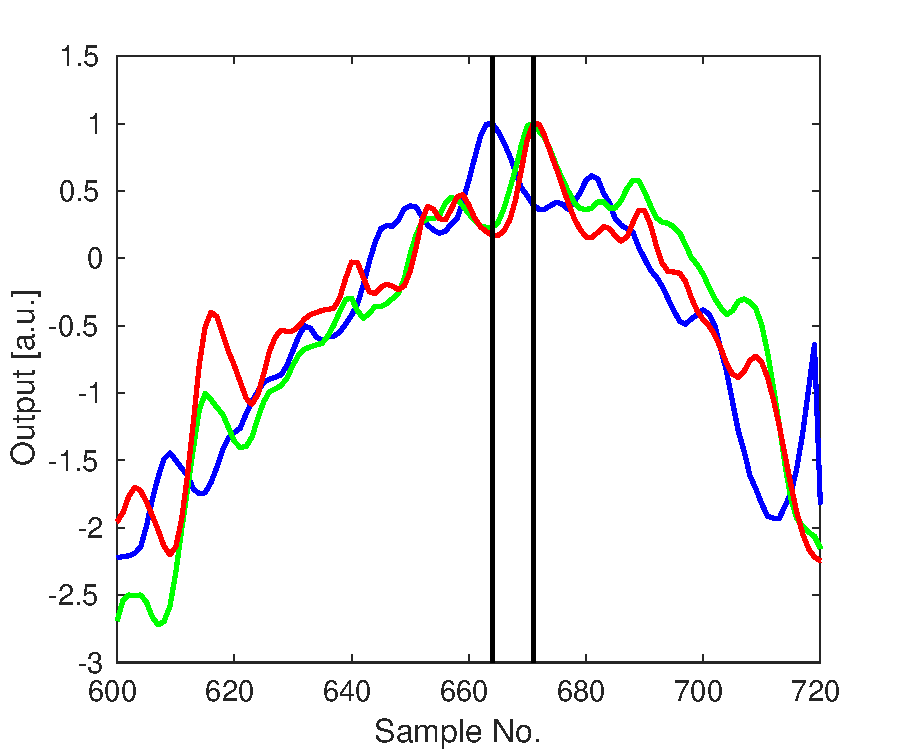
\includegraphics[width=0.9\textwidth]{Figures/commissioning/absTimBeam_d0}
  \caption{Kick output with no delay as seen on BPM and phase signals.}
  \label{f:absTimBeam_d0}
\end{figure}

This measurement was repeated with four different correction output delays applied in the FONT5 board, at delays of 0, 10, 20 and 30~clock~cycles (0 to 84~ns), which includes points where the correction is applied both early and late. Fitting the measured time offset between the peaks in the BPM and the phase in the same way as before yields an optimal correction output delay to apply of \(39\pm7\)~ns (Figure \ref{f:absTimBeam_fit}), or \(14\pm3\)~clock~cycles. Applying this delay in data analysis gives the result shown in Figure~\ref{f:absTimBeam_opt}, in which the similarity of the three signals becomes clear.

\begin{figure}
  \centering
  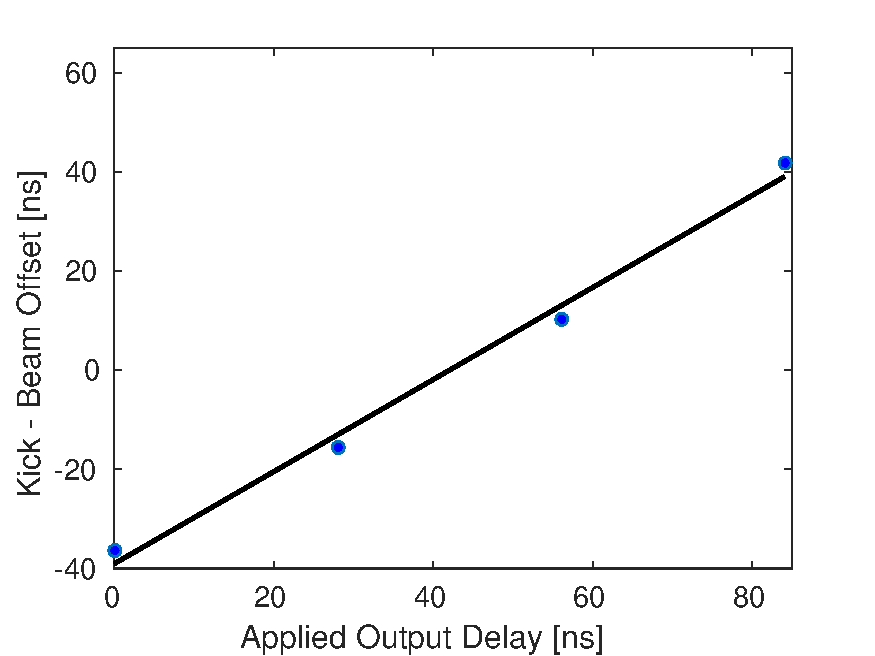
\includegraphics[width=0.9\textwidth]{Figures/commissioning/absTimBeam_fit}
  \caption{Fit time offset between kick and beam at different output delays.}
  \label{f:absTimBeam_fit}
\end{figure}

\begin{figure}
  \centering
  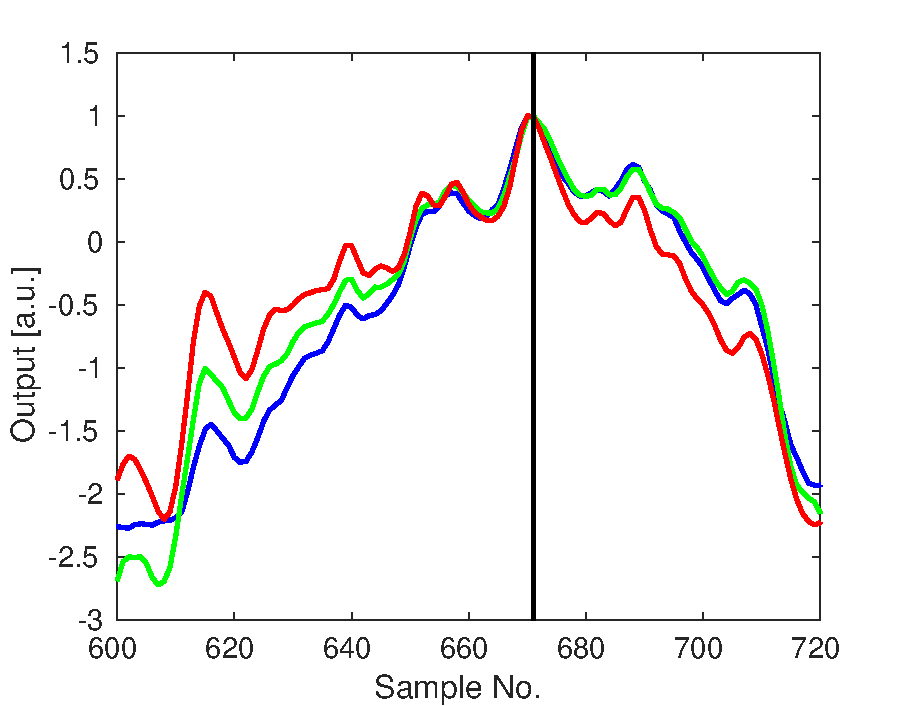
\includegraphics[width=0.9\textwidth]{Figures/commissioning/absTimBeam_opt}
  \caption{Alignment between BPMs and phase signals with optimal delay applied in analysis.}
  \label{f:absTimBeam_opt}
\end{figure}


\subsection{Relative Kicker Timing}
\label{ss:relativeTiming}


offset calculated first slope: \(1.9\pm2.0\)~clock~cycles
offset calculated second slope: \(0.13\pm0.51\)~clock~cycles (better data)

\begin{figure}
  \centering
  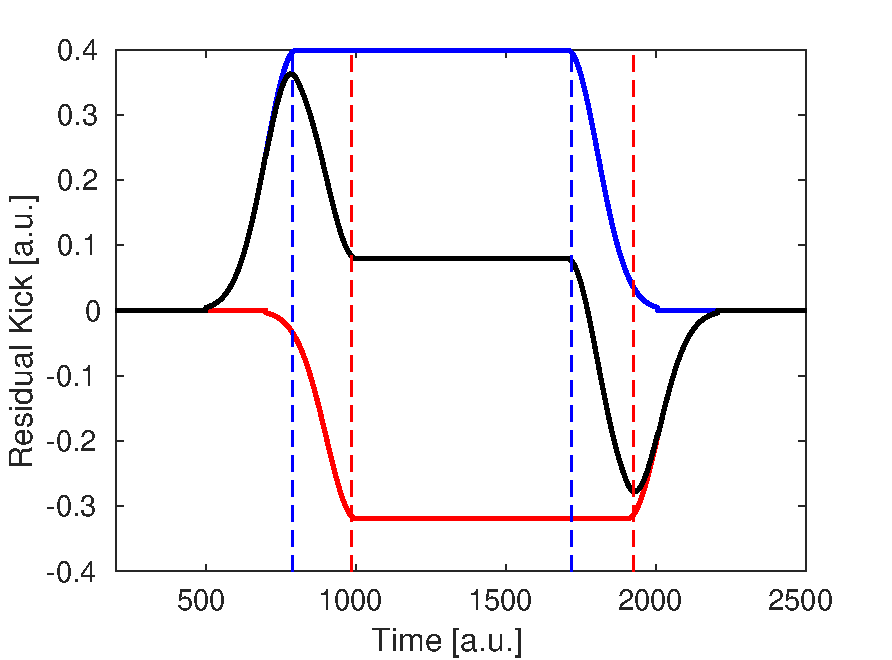
\includegraphics[width=0.9\textwidth]{Figures/commissioning/relDelay_sim}
  \caption{Simulated response to offset kicks.}
  \label{f:relDelay_sim}
\end{figure}

\begin{figure}
  \centering
  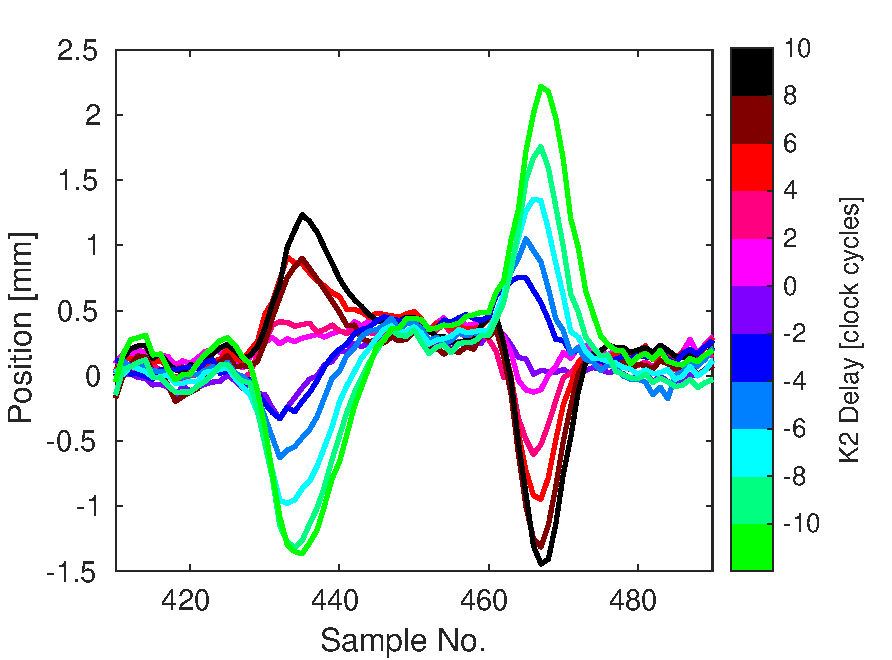
\includegraphics[width=0.9\textwidth]{Figures/commissioning/relDelay_traces}
  \caption{Measured BPM offset for different relative kick delays.}
  \label{f:relDelay_traces}
\end{figure}

\begin{figure}
  \centering
  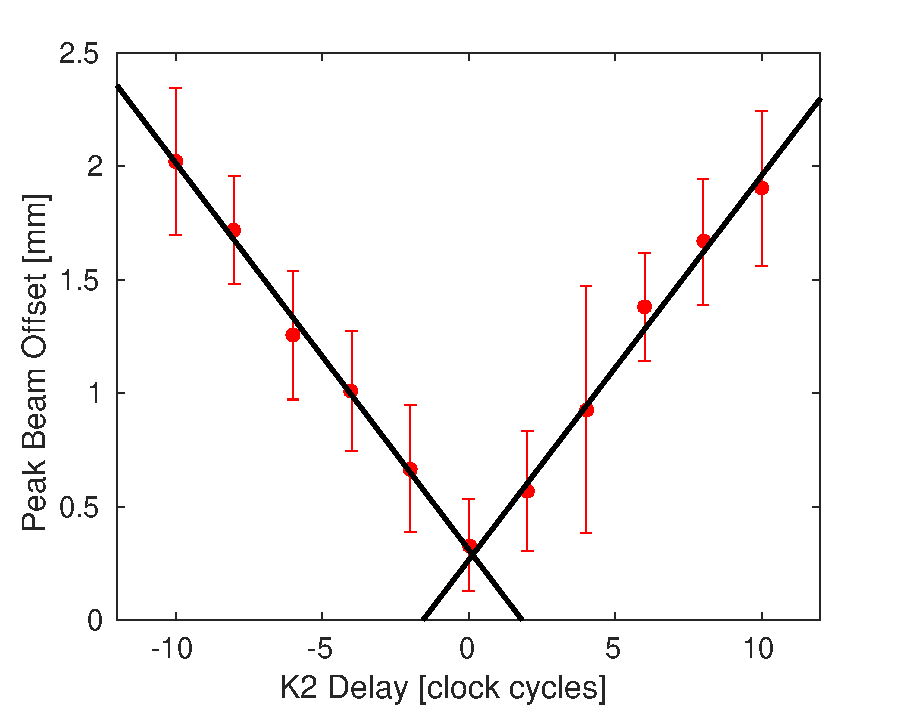
\includegraphics[width=0.9\textwidth]{Figures/commissioning/relDelay_fit}
  \caption{Fitted peak BPM offset vs. relative kick delay.}
  \label{f:relDelay_sim}
\end{figure}



%\newsection{corrBandwidth}{Correction Bandwidth}




